\begin{homeworkProblem}
Let $X_1 , \ldots ,X_n \mathop \sim\limits^{i.i.d.} N\left( {\mu 
,\sigma ^2 } \right)$.
We will use the generalized likilihood ratio method to construct a test for the hypotheses:
\[
\begin{array}{*{20}c}
   {H_0 :\mu  \leqslant 5} & {{\text{vs}}{\text{.}}} & {H_1 :\mu  > 5}  
\\

 \end{array} 
\]
The likilihood function is given by:
\[
L = \prod\limits_{i = 1}^n {\frac{1}
{{\sqrt {2\pi \sigma ^2 } }}\exp \left\{ { - \frac{{\left( {x_i  - \mu } \right)^2 }}
{{2\sigma ^2 }}} \right\} = } \left( {2\pi \sigma ^2 } \right)^{ - \frac{n}
{2}} \exp \left\{ { - \frac{1}
{{2\sigma ^2 }}\sum\limits_{i = 1}^n {\left( {x_i  - \mu } \right)^2 } } \right\}
\]
The log-likilihood function is therefore:
\[
LL =  - \frac{n}
{2}\ln \left( {2\pi } \right) - \frac{n}
{2}\ln \left( {\sigma ^2 } \right) - \frac{1}
{{2\sigma ^2 }}\sum\limits_{i = 1}^n {\left( {x_i  - \mu } \right)^2 } 
\]
Computing the MLEs ${\hat \mu ,\hat \sigma ^2 }$ gives:
\[
\frac{{\partial LL}}
{{\partial \mu }} = 0 \Rightarrow \sum\limits_{i = 1}^n {x_i  - n\mu  = 0}  \Rightarrow \hat \mu  = \bar X_n 
\]
\[
\frac{{\partial LL}}
{{\partial \sigma ^2 }} = 0 \Rightarrow  - \frac{n}
{{2\sigma ^2 }} - \frac{1}
{{2\left( {\sigma ^2 } \right)^2 }}\sum\limits_{i = 1}^n {\left( {x_i  - \hat \mu } \right)^2 }  = 0 \Rightarrow \hat \sigma ^2  = \frac{1}
{n}\sum\limits_{i = 1}^n {\left( {x_i  - \bar X_n } \right)^2 } 
\]
The MLEs ${\tilde \mu ,\tilde \sigma ^2 }$ constrained by the null hypothesis will be identical to ${\hat \mu ,\hat \sigma ^2 }$ if $\bar X_n \le 5$; and $\tilde \mu  = 5,\hat \sigma ^2  = \frac{1}{n}\sum\limits_{i = 1}^n {\left( {x_i  - 5} \right)^2 }$ otherwise. If the two sets of MLEs are identical, then $\Lambda=1$, and we would never reject $H_0$. Therefore, to determine a decision rule for rejection, we may just consider the case where $\tilde \mu  = 5,\hat \sigma ^2  = \frac{1}{n}\sum\limits_{i = 1}^n {\left( {x_i  - 5} \right)^2 }$. From our MLEs, $\Lambda$ is given by:
\[
\Lambda  = \frac{{L\left( {\tilde \mu ,\tilde \sigma ^2 } \right)}}
{{L\left( {\hat \mu ,\hat \sigma ^2 } \right)}} = \frac{{\left( {2\pi \tilde \sigma ^2 } \right)^{ - \frac{n}
{2}} \exp \left\{ { - \frac{1}
{{2\tilde \sigma ^2 }}\sum\limits_{i = 1}^n {\left( {x_i  - 5} \right)^2 } } \right\}}}
{{\left( {2\pi \hat \sigma ^2 } \right)^{ - \frac{n}
{2}} \exp \left\{ { - \frac{1}
{{2\hat \sigma ^2 }}\sum\limits_{i = 1}^n {\left( {x_i  - \bar X_n } \right)^2 } } \right\}}} = \left( {\frac{{2\pi \hat \sigma ^2 }}
{{2\pi \tilde \sigma ^2 }}} \right)^{\frac{n}
{2}} 
\]
\[
 = \left( {\frac{{2\pi \frac{1}
{n}\sum\limits_{i = 1}^n {\left( {x_i  - \bar X_n } \right)^2 } }}
{{2\pi \frac{1}
{n}\sum\limits_{i = 1}^n {\left( {x_i  - 5} \right)^2 } }}} \right)^{\frac{n}
{2}}  = \left( {\frac{{\sum\limits_{i = 1}^n {\left( {x_i  - \bar X_n } \right)^2 } }}
{{\sum\limits_{i = 1}^n {\left( {x_i  - 5} \right)^2 } }}} \right)^{\frac{n}
{2}} 
\]
Our decision rule is to reject $H_0$ if and only if $\Lambda<c\le 1$ where is is determined by $P_{\mu  \leqslant 5} \left( {\Lambda  < c} \right) = \alpha$. Manipulation of the test statistic and decision rule gives:
\[
\left( {\frac{{\sum\limits_{i = 1}^n {\left( {x_i  - \bar X_n } \right)^2 } }}
{{\sum\limits_{i = 1}^n {\left( {x_i  - 5} \right)^2 } }}} \right)^{\frac{n}
{2}}  < c \Rightarrow \left( {\frac{{\sum\limits_{i = 1}^n {\left( {x_i  - 5} \right)^2 } }}
{{\sum\limits_{i = 1}^n {\left( {x_i  - \bar X_n } \right)^2 } }}} \right)^{\frac{n}
{2}}  > c' \Rightarrow \frac{{\sum\limits_{i = 1}^n {\left( {x_i  - \bar X_n  + \bar X_n  - 5} \right)^2 } }}
{{\sum\limits_{i = 1}^n {\left( {x_i  - \bar X_n } \right)^2 } }} \geqslant c''
\]
\[
 \Rightarrow \frac{{\sum\limits_{i = 1}^n {\left( {x_i  - \bar X_n } \right)^2 }  + 2\sum\limits_{i = 1}^n {\left( {x_i  - \bar X_n } \right)\left( {\bar X_n  - 5} \right)}  + \sum\limits_{i = 1}^n {\left( {\bar X_n  - 5} \right)^2 } }}
{{\sum\limits_{i = 1}^n {\left( {x_i  - \bar X_n } \right)^2 } }} > c'''
\]
\[
 \Rightarrow \frac{{\sum\limits_{i = 1}^n {\left( {x_i  - \bar X_n } \right)^2 }  + n\left( {\bar X_n  - 5} \right)}}
{{\sum\limits_{i = 1}^n {\left( {x_i  - \bar X_n } \right)^2 } }} > c''' \Rightarrow 1 + \frac{{n\left( {\bar X_n  - 5} \right)^2 }}
{{\sum\limits_{i = 1}^n {\left( {x_i  - \bar X_n } \right)^2 } }} > c''''
\]
\[
 \Rightarrow \frac{{\left( {\bar X_n  - 5} \right)}}
{{\sqrt {\sum\limits_{i = 1}^n {\left( {x_i  - \bar X_n } \right)^2 /n} } }} > c''''' \Rightarrow \frac{u}
{{\sqrt {V/d} }}\sim T\left( {n - 1} \right)
\]
So, the simplified test statistic $\frac{{\sqrt n \left( {\bar X_n  - 5} \right)}}{S}$ is recognized as having a Student's T distribution with $n-1$ degrees of freedom.
Therefore, the test function may be written as:
\[
\phi \left( {Z_1 , \ldots ,Z_n } \right) = \left\{ {\begin{array}{*{20}c}
   1 & {{\text{if }}\bar X_n  > 5 + \frac{{C_{0.05,n - 1} S}}
{{\sqrt n }}}  \\
   0 & {o.w.}  \\

 \end{array} } \right.
\]
where $C_{0.05,n - 1}$ is determined from the Student's T distribtion with $n-1$ degrees of freedom such that the area under the density to the right of $t=C_{0.05,n - 1}$ has an area of $0.05=\alpha$.
\end{homeworkProblem}

\begin{homeworkProblem}
Let $Y_i  = \alpha  + \beta x_i  + \varepsilon _i ,i = 1,2, \ldots 
,n$, with $\varepsilon _1 , \ldots ,\varepsilon _n \mathop \sim 
\limits^{{\text{iid}}} N\left( {0,\sigma ^2 } \right)$ and $\sigma^2$ 
is unknown. Assume $n \ge 3$. It is required to find a generalized 
likelihood ratio test for: 
\[
\begin{array}{*{20}c}
   {H:\beta  \leqslant \beta _0 } & {{\text{vs}}{\text{.}}} & {K:\beta  
> \beta _0 }  \\

 \end{array} 
\]
Since $Y_i \sim N\left( {\alpha  + \beta x_i ,\sigma ^2 } \right)$, 
the likelihood function is given by:
\[
L = \prod\limits_{i = 1}^n {\frac{1}
{{\sqrt {2\pi \sigma ^2 } }}\exp \left\{ { - \frac{1}
{{2\sigma ^2 }}\left( {y_i  - \left( {\alpha  + \beta x_i } \right)} 
\right)^2 } \right\}} 
\]
\[
 = \left( {2\pi \sigma ^2 } \right)^{ - \frac{n}
{2}} \exp \left\{ { - \frac{1}
{{2\sigma ^2 }}\sum\limits_{i = 1}^n {\left[ {y_i  - \left( {\alpha  + 
\beta x_i } \right)} \right]^2 } } \right\}
\]
So, the log-likelihood function is given as:
\[
\ln \left( L \right) =  - \frac{n}
{2}\ln \left( {2\pi } \right) - \frac{n}
{2}\ln \left( {\sigma ^2 } \right) - \frac{1}
{{2\sigma ^2 }}\sum\limits_{i = 1}^n {\left[ {y_i  - \left( {\alpha  + 
\beta x_i } \right)} \right]^2 } 
\]
The MLEs for $\alpha ,\beta ,\sigma ^2$ are found by simultaneously 
solving:
\[
\left\{ {\begin{array}{*{20}c}
   {\frac{{\partial \ln \left( L \right)}}
{{\partial \alpha }} = 0}  \\
   {\frac{{\partial \ln \left( L \right)}}
{{\partial \beta }} = 0}  \\
   {\frac{{\partial \ln \left( L \right)}}
{{\partial \sigma ^2 }} = 0}  \\

 \end{array} } \right. \Rightarrow \left\{ {\begin{array}{*{20}c}
   {\frac{1}
{{\sigma ^2 }}\sum\limits_{i = 1}^n {\left[ {y_i  - \left( {\alpha  + 
\beta x_i } \right)} \right]}  = 0}  \\
   {\frac{1}
{{\sigma ^2 }}\sum\limits_{i = 1}^n {x_i \left[ {y_i  - \left( {\alpha  
+ \beta x_i } \right)} \right]}  = 0}  \\
   {\frac{1}
{{2\sigma ^2 }}\sum\limits_{i = 1}^n {\left[ {y_i  - \left( {\alpha  + 
\beta x_i } \right)} \right]^2 }  - \frac{n}
{{2\sigma ^2 }} = 0}  \\

 \end{array} } \right.
\]
\[
 \Rightarrow \left\{ {\begin{array}{*{20}c}
   {\frac{1}
{n}\sum\limits_{i = 1}^n {y_i }  - \frac{1}
{n}n\alpha  - \frac{\beta }
{n}\sum\limits_{i = 1}^n {x_i }  = 0}  \\
   {\frac{{\sum\limits_{i = 1}^n {y_i \left( {x_i  - \bar X_n } 
\right)} }}
{{\sum\limits_{i = 1}^n {\left( {x_i  - \bar X_n } \right)^2 } }} - 
\beta  = 0}  \\
   {\frac{1}
{n}\sum\limits_{i = 1}^n {\left[ {y_i  - \left( {\alpha  + \beta x_i } 
\right)} \right]^2  - \sigma ^2  = 0} }  \\

 \end{array} } \right. \Rightarrow \left\{ {\begin{array}{*{20}c}
   \begin{gathered}
  \hat \alpha  = \bar Y_n  - \hat \beta \bar X_n  \hfill \\
   \hfill \\ 
\end{gathered}   \\
   {\hat \beta  = \frac{{\sum\limits_{i = 1}^n {\left( {y_i  - \bar 
Y_n } \right)\left( {x_i  - \bar X_n } \right)} }}
{{\sum\limits_{i = 1}^n {\left( {x_i  - \bar X_n } \right)^2 } }}}  \\
   {\hat \sigma ^2  =   \frac{1}
{n}\sum\limits_{i = 1}^n {\left[ {y_i  - \left( {\hat \alpha  + \hat 
\beta x_i } \right)} \right]^2 } }  \\

 \end{array} } \right.
\]
The MLEs for $\alpha ,\beta ,\sigma ^2$ restricted to ${\beta  
\leqslant \beta _0 }$ are therefore given as:

\[
{\text{if }}\frac{{\sum\limits_{i = 1}^n {\left( {y_i  - \bar Y_n } 
\right)\left( {x_i  - \bar X_n } \right)} }}
{{\sum\limits_{i = 1}^n {\left( {x_i  - \bar X_n } \right)^2 } }} 
\leqslant \beta _0 {\text{, then: }}\left\{ {\begin{array}{*{20}c}
   \begin{gathered}
  \hat \alpha _H  = \bar Y_n  - \hat \beta _H \bar X_n  \hfill \\
   \hfill \\ 
\end{gathered}   \\
   {\hat \beta _H  = \frac{{\sum\limits_{i = 1}^n {\left( {y_i  - \bar 
Y_n } \right)\left( {x_i  - \bar X_n } \right)} }}
{{\sum\limits_{i = 1}^n {\left( {x_i  - \bar X_n } \right)^2 } }}}  \\
   {\hat \sigma ^2 _H  =   \frac{1}
{n}\sum\limits_{i = 1}^n {\left[ {y_i  - \left( {\hat \alpha _H  + 
\hat \beta _H x_i } \right)} \right]^2 } }  \\

 \end{array} } \right.
\]
\[
{\text{otherwise: }}\left\{ {\begin{array}{*{20}c}
   {\hat \alpha _H  = \bar Y_n  - \hat \beta _H \bar X_n }  \\
   {\hat \beta _H  = \beta _0 }  \\
   {\hat \sigma _H^2  =   \frac{1}
{n}\sum\limits_{i = 1}^n {\left[ {y_i  - \left( {\hat \alpha _H  + 
\hat \beta _H x_i } \right)} \right]^2 } }  \\

 \end{array} } \right.
\]

The likelihood ratio test is constructed by forming:
\[
\Lambda  = \frac{{L\left( {\hat \alpha _H ,\hat \beta _H ,\hat \sigma 
^2 _H } \right)}}
{{L\left( {\hat \alpha ,\hat \beta ,\hat \sigma ^2 } \right)}}
\]
and we reject the null hypothesis $H$ if $\Lambda  < c_\alpha \le 
1$\footnote{Here $\alpha$ represents the selected level of 
significance of the test, not the additive constant regression 
parameter} for some $c_\alpha$ determined by $P\left( {\Lambda  < 
c_\alpha  } \right) = \alpha$. So, in the case where 
$\frac{{\sum\limits_{i = 1}^n {\left( {y_i  - \bar Y_n } \right)\left( 
{x_i  - \bar X_n } \right)} }}{{\sum\limits_{i = 1}^n {\left( {x_i  - 
\bar X_n } \right)^2 } }} \leqslant \beta _0$, we will never reject 
$H$. Therefore, we construct the numerator of $\Lambda$ using the 
restricted MLEs given by:
\[
\left\{ {\begin{array}{*{20}c}
   {\hat \alpha _H  = \bar Y_n  - \hat \beta _H \bar X_n }  \\
   {\hat \beta _H  = \beta _0 }  \\
   {\hat \sigma _H^2  =   \frac{1}
{n}\sum\limits_{i = 1}^n {\left[ {y_i  - \left( {\hat \alpha _H  + 
\hat \beta _H x_i } \right)} \right]^2 } }  \\

 \end{array} } \right.
\]
Plugging these values in gives:
\[
\Lambda  = \frac{{L\left( {\hat \alpha _H ,\hat \beta _H ,\hat \sigma 
^2 _H } \right)}}
{{L\left( {\hat \alpha ,\hat \beta ,\hat \sigma ^2 } \right)}} = 
\frac{{\left. {\left( {2\pi \sigma ^2 } \right)^{ - \frac{n}
{2}} \exp \left\{ { - \frac{1}
{{2\sigma ^2 }}\sum\limits_{i = 1}^n {\left[ {y_i  - \left( {\alpha  + 
\beta x_i } \right)} \right]^2 } } \right\}} \right|_{\left( {\alpha 
,\beta ,\sigma ^2 } \right) = \left( {\hat \alpha _H ,\hat \beta _H 
,\hat \sigma ^2 _H } \right)} }}
{{\left. {\left( {2\pi \sigma ^2 } \right)^{ - \frac{n}
{2}} \exp \left\{ { - \frac{1}
{{2\sigma ^2 }}\sum\limits_{i = 1}^n {\left[ {y_i  - \left( {\alpha  + 
\beta x_i } \right)} \right]^2 } } \right\}} \right|_{\left( {\alpha 
,\beta ,\sigma ^2 } \right) = \left( {\hat \alpha ,\hat \beta ,\hat 
\sigma ^2 } \right)} }}
\]
\[
 = \frac{{\left( {2\pi \frac{1}
{n}\sum\limits_{i = 1}^n {\left[ {y_i  - \left( {\left[ {\bar Y_n  - 
\beta _0 \bar X_n } \right] + \beta _0 x_i } \right)} \right]^2 } } 
\right)^{ - \frac{n}
{2}} }}
{{\left( {2\pi \frac{1}
{n}\sum\limits_{i = 1}^n {\left[ {y_i  - \left( {\left[ {\bar Y_n  - 
\frac{{\sum\limits_{i = 1}^n {\left( {y_i  - \bar Y_n } \right)\left( 
{x_i  - \bar X_n } \right)} }}
{{\sum\limits_{i = 1}^n {\left( {x_i  - \bar X_n } \right)^2 } }}\bar 
X} \right] + \frac{{\sum\limits_{i = 1}^n {\left( {y_i  - \bar Y_n } 
\right)\left( {x_i  - \bar X_n } \right)} }}
{{\sum\limits_{i = 1}^n {\left( {x_i  - \bar X_n } \right)^2 } }}x_i } 
\right)} \right]^2 } } \right)^{ - \frac{n}
{2}} }}
\]
\[
 = \left( {\frac{{\sum\limits_{i = 1}^n {\left[ {y_i  - \left( {\left[ 
{\bar Y_n  - \beta _0 \bar X_n } \right] + \beta _0 x_i } \right)} 
\right]^2 } }}
{{\sum\limits_{i = 1}^n {\left[ {y_i  - \left( {\left[ {\bar Y_n  - 
b_1 \bar X} \right] + b_1 x_i } \right)} \right]^2 } }}} 
\right)^{\frac{n}
{2}} 
\]
where $b_1  = \frac{{\sum\limits_{i = 1}^n {\left( {y_i  - \bar Y_n } 
\right)\left( {x_i  - \bar X_n } \right)} }}{{\sum\limits_{i = 1}^n 
{\left( {x_i  - \bar X_n } \right)^2 } }}$.
Manipulation of the expression and corresponding decision rule gives:
\[
\left( {\frac{{\sum\limits_{i = 1}^n {\left[ {\left( {y_i  - \bar Y_n 
} \right) - \beta _0 \left( {x_i  - \bar X_n } \right)} \right]^2 } }}
{{\sum\limits_{i = 1}^n {\left[ {\left( {y_i  - \bar Y_n } \right) - 
b_1 \left( {x_i  - \bar X_n } \right)} \right]^2 } }}} 
\right)^{\frac{n}
{2}}  < c_\alpha   \Rightarrow \frac{{\sum\limits_{i = 1}^n {\left[ 
{\left( {y_i  - \bar Y_n } \right) - \beta _0 \left( {x_i  - \bar X_n 
} \right)} \right]^2 } }}
{{\sum\limits_{i = 1}^n {\left[ {\left( {y_i  - \bar Y_n } \right) - 
b_1 \left( {x_i  - \bar X_n } \right)} \right]^2 } }} < c_\alpha 
^{'}\]
Since ${\left( {y_i  - \bar Y_n } \right) - \beta _0 \left( {x_i  - 
\bar X_n } \right)}$ is normally distributed for each $i$, and it is 
given that $\frac{1}{{\sigma ^2 }}\sum\limits_{i = 1}^n {\left[ 
{\left( {y_i  - \bar Y_n } \right) - b_1 \left( {x_i  - \bar X_n } 
\right)} \right]^2 } \sim \chi _{\left( {n - 2} \right)}^2$, the test 
statistic (with appropriate constant scalings) has the form 
$\frac{{Z^2 }}{{V/D}}$, with $Z\sim N\left( {0,1} \right)$ and $V\sim 
\chi _{\left( {d = n - 2} \right)}^2$. This can also be written as:
\[
\frac{{\chi _{\left( 1 \right)}^2 /1}}
{{\chi _{\left( {n - 2} \right)}^2 /\left( {n - 2} \right)}}\sim 
F\left( {1,n - 2} \right)
\]
in which case our test statistic has an $F$ distribution. Since the 
numerator and denominator of our test statistic are both positive, we 
may also compute the square root and obtain a statistic of the form:
\[
\frac{Z}
{{\sqrt {\chi _{\left( {n - 2} \right)}^2 /\left( {n - 2} \right)} 
}}\sim {\text{StudentT}}\left( {n - 2} \right)
\]
in which case our test statistic has a Student's $T$ distribution. For 
this choice, we would reject $H$ in favor of $K$ if $\phi \left( 
{\underset{\raise0.3em\hbox{$\smash{\scriptscriptstyle\thicksim}$}}{X} 
,\underset{\raise0.3em\hbox{$\smash{\scriptscriptstyle\thicksim}$}}{Y} 
} \right)=1$, where:
\[
\phi \left( 
{\underset{\raise0.3em\hbox{$\smash{\scriptscriptstyle\thicksim}$}}{X} 
,\underset{\raise0.3em\hbox{$\smash{\scriptscriptstyle\thicksim}$}}{Y} 
} \right) = \left\{ {\begin{array}{*{20}c}
   1 & {t < c}  \\
   0 & {o.w.}  \\

 \end{array} } \right.
\]
\[
t = \frac{{\sum\limits_{i = 1}^n {\left[ {\left( {y_i  - \bar Y_n } 
\right) - \beta _0 \left( {x_i  - \bar X_n } \right)} \right]} }}
{{\sum\limits_{i = 1}^n {\left[ {\left( {y_i  - \bar Y_n } \right) - 
b_1 \left( {x_i  - \bar X_n } \right)} \right]} }}
\]
and $c$ is the constant such that $1 - \int_{ - \infty}^{c} {f_T } dt 
= \alpha$ for some level of significance $\alpha$ with $f_T$ being the 
density of the Student's T distribution with $n-2$ degrees of freedom. 
For this problem (as well as the problems which follow) the density 
function of the test statistic was estimated using a 100,000 iteration (with 15,000 samples each) Monte-Carlo simulation, sorted into 50 categorical bins on the number line. 
\begin{figurehere}
\centering
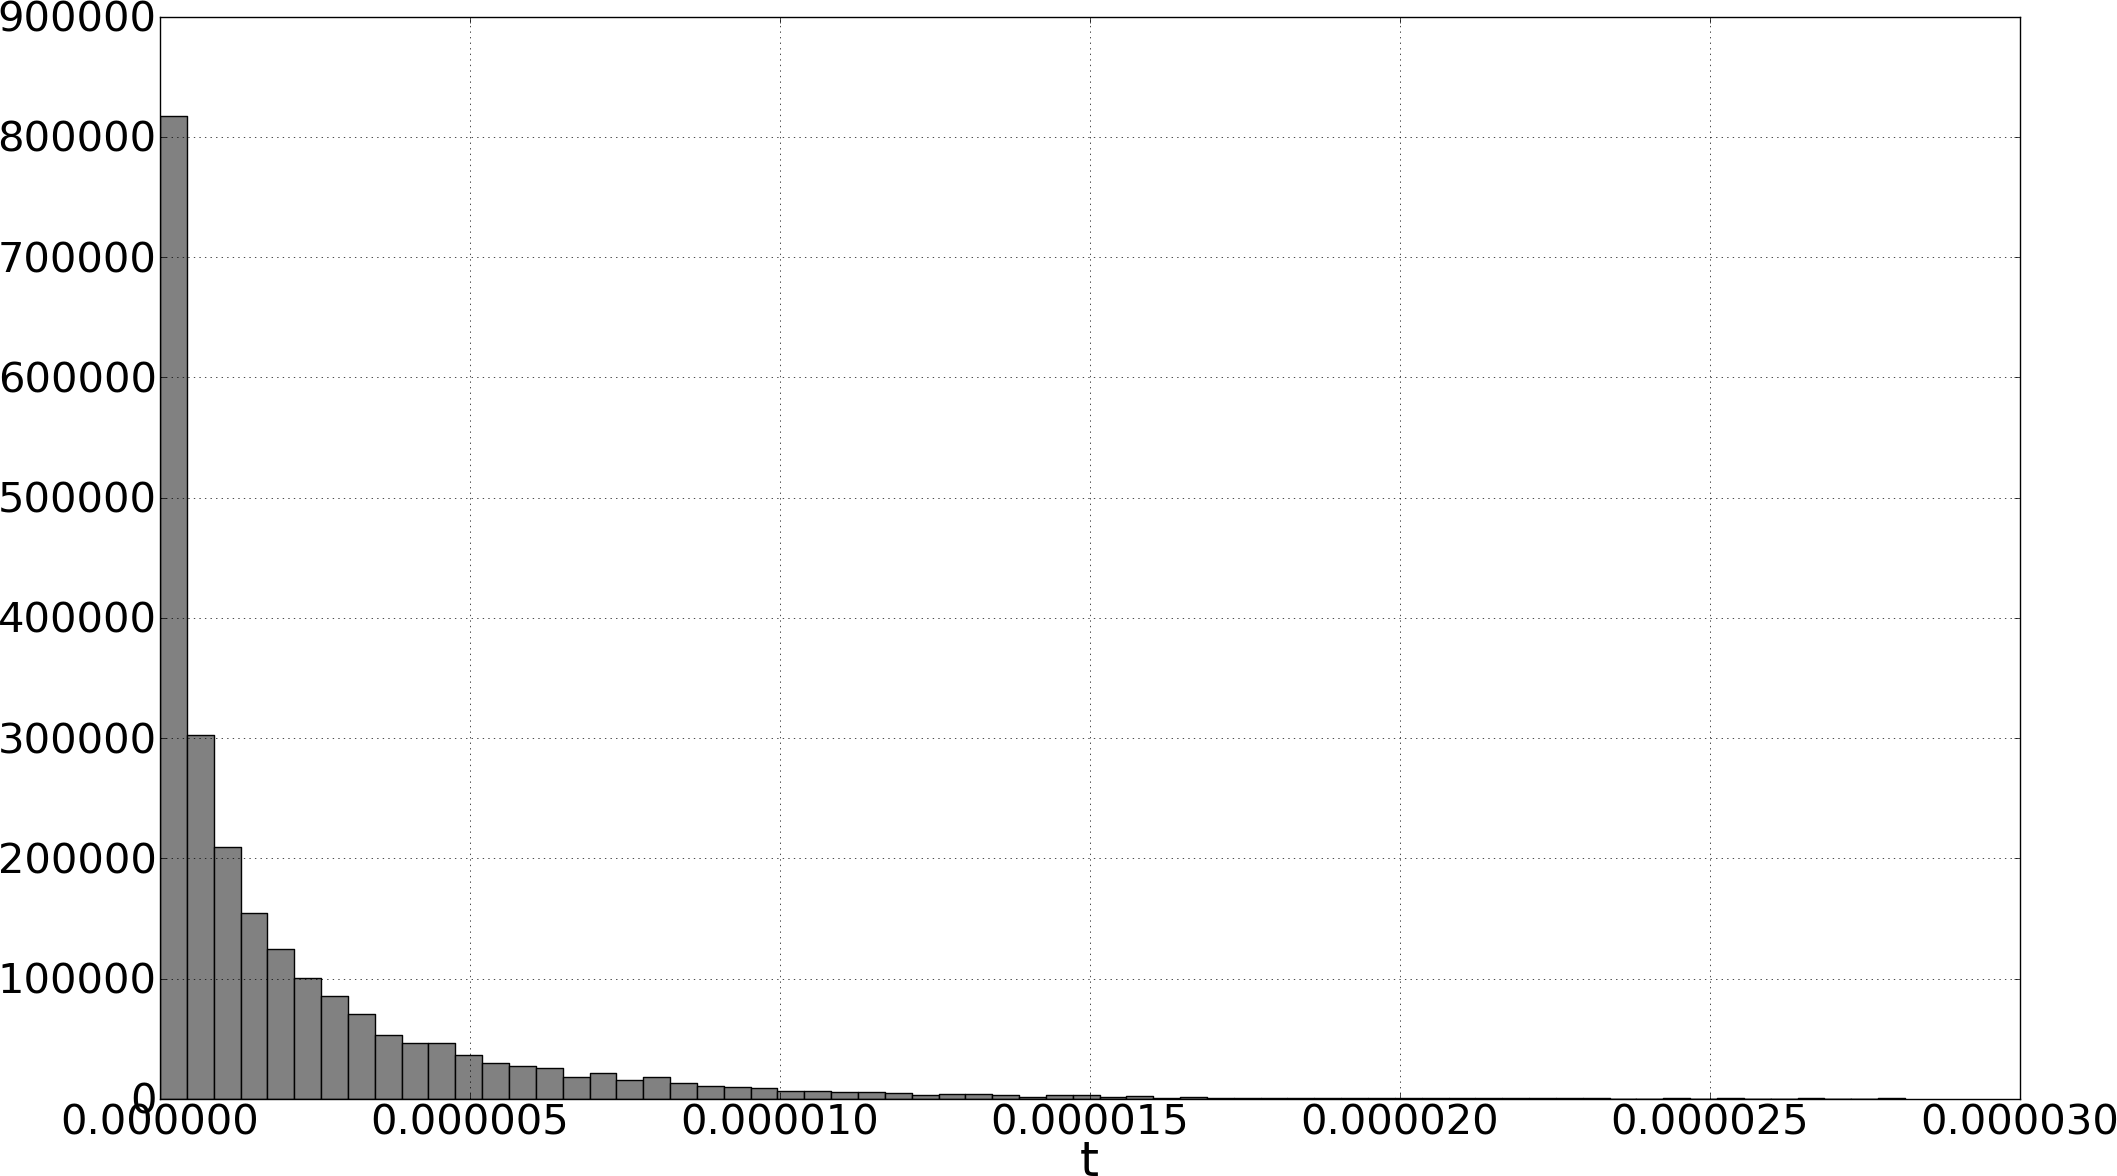
\includegraphics[width=.98\columnwidth]{57f.png}
\caption{A plot of the simulated density of the test statistic for 
Problem 57, without computation of a square-root. This appears to have 
the shape of an $F-$distribution.}
\end{figurehere}
\begin{figurehere}
\centering
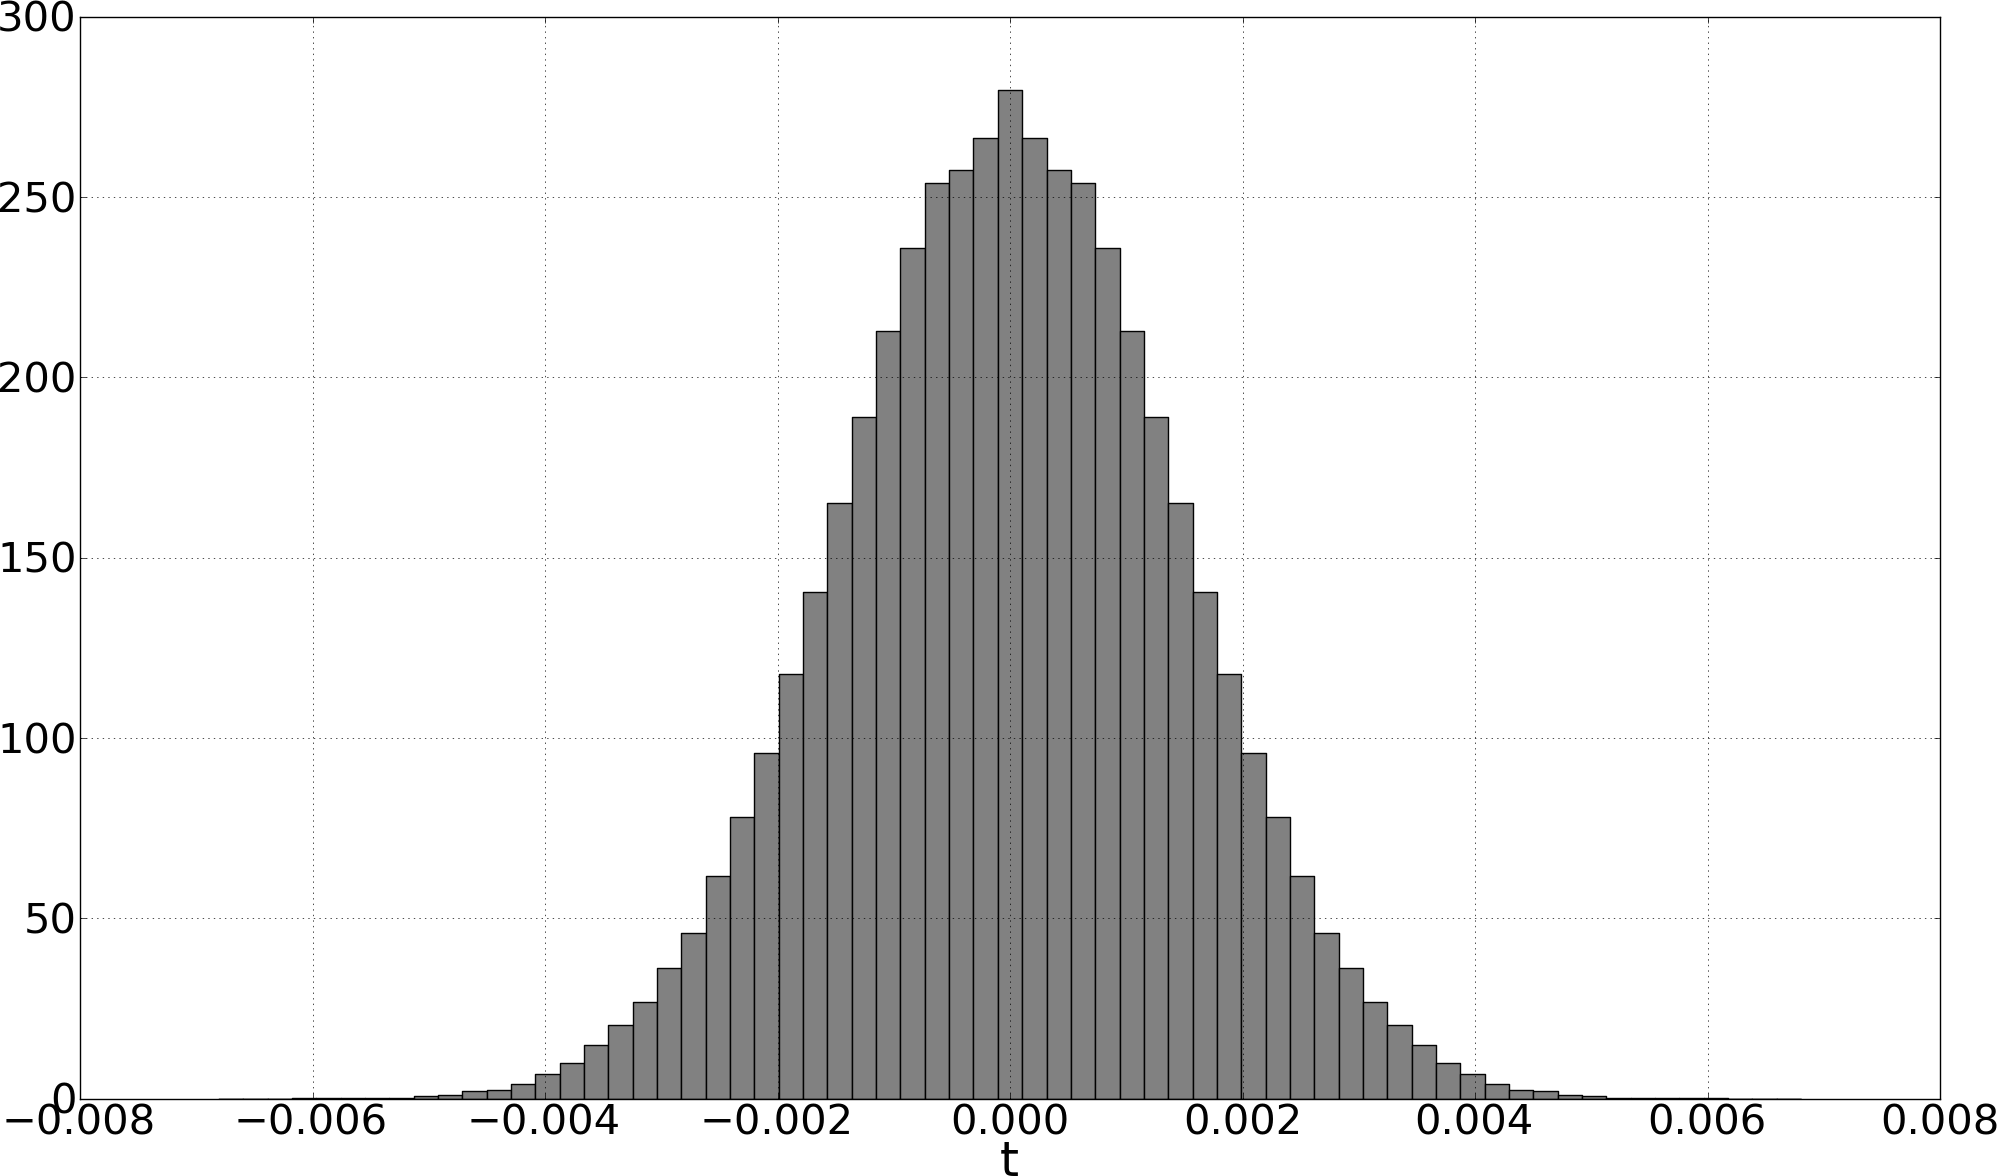
\includegraphics[width=.98\columnwidth]{57t.png}
\caption{A plot of the simulated density of the test statistic for 
Problem 57, with the computation of the square root. For this plot, 
the histogram was reflected about 0 to induce the proper symmetry. 
This appears to have the shape of a student's $T-$distribution, as 
expected.}
\end{figurehere}
\end{homeworkProblem}

\begin{homeworkProblem}
It is given that $X_1 , \ldots ,X_m \sim N\left( {\mu _1 ,\sigma _1^2 
} \right)$ and $Y_1 , \ldots ,Y_n \sim N\left( {\mu _2 ,\sigma _2^2 } 
\right)$, with all parameters unknown. The objective is to formulate a 
generalized likelihood ratio test for equality of variance:
\[
\begin{array}{*{20}c}
   {H:\Delta  = \Delta _0 } & {vs.} & {K:\Delta  \ne \Delta _0 }  \\

 \end{array} 
\]
with $\Delta  = \frac{{\sigma _2^2 }}{{\sigma _1^2 }}$.
The likelihood function is given by:
\[
L = \left[ {\prod\limits_{i = 1}^m {\frac{1}
{{\sqrt {2\pi \sigma _1^2 } }}\exp \left\{ { - \frac{1}
{{2\sigma _1^2 }}\left( {x_i  - \mu _1 } \right)^2 } \right\}} } 
\right]\left[ {\prod\limits_{j = 1}^n {\frac{1}
{{\sqrt {2\pi \sigma _2^2 } }}\exp \left\{ { - \frac{1}
{{2\sigma _2^2 }}\left( {y_j  - \mu _2 } \right)^2 } \right\}} } 
\right]
\]
\[
 = \left( {2\pi \sigma _1^2 } \right)^{ - \frac{m}
{2}} \exp \left\{ { - \frac{1}
{{2\sigma _1^2 }}\sum\limits_{i = 1}^m {\left( {x_1  - \mu _1 } 
\right)^2 } } \right\}\left( {2\pi \sigma _2^2 } \right)^{ - \frac{n}
{2}} \exp \left\{ { - \frac{1}
{{2\sigma _2^2 }}\sum\limits_{j = 1}^n {\left( {y_j  - \mu _2 } 
\right)^2 } } \right\}
\]
\[
 = \left( {2\pi } \right)^{ - \frac{{m + n}}
{2}} \left( {\sigma _1^2 } \right)^{ - \frac{m}
{2}} \left( {\sigma _2^2 } \right)^{ - \frac{n}
{2}} \exp \left\{ { - \frac{1}
{{2\sigma _1^2 }}\sum\limits_{i = 1}^m {\left( {x_1  - \mu _1 } 
\right)^2 }  - \frac{1}
{{2\sigma _2^2 }}\sum\limits_{j = 1}^n {\left( {y_j  - \mu _2 } 
\right)^2 } } \right\}
\]
The log-likelihood function is therefore computed to be:
\[
LL =  - \frac{{m + n}}
{2}\ln \left( {2\pi } \right) - \frac{m}
{2}\ln \left( {\sigma _1^2 } \right) - \frac{n}
{2}\ln \left( {\sigma _2^2 } \right) - \frac{1}
{{2\sigma _1^2 }}\sum\limits_{i = 1}^m {\left( {x_i  - \mu _1 } 
\right)^2 }  - \frac{1}
{{2\sigma _2^2 }}\sum\limits_{j = 1}^n {\left( {y_j  - \mu _2 } 
\right)^2 } 
\]
Solving for the MLEs $\hat \mu _1 ,\hat \mu _2 ,\hat \sigma _1^2,\hat 
\sigma _2^2$ gives:
\[
\frac{{\partial LL}}
{{\partial \mu _1 }} = 0 \Rightarrow \frac{1}
{{\sigma _1^2 }}\sum\limits_{i = 1}^m {\left( {x_i  - \mu _1 } 
\right)}  = 0 \Rightarrow \hat \mu _1  = \bar X_m 
\]
\[
\frac{{\partial LL}}
{{\partial \mu _2 }} = 0 \Rightarrow \frac{1}
{{\sigma _2^2 }}\sum\limits_{i = 1}^n {\left( {y_i  - \mu _2 } 
\right)}  = 0 \Rightarrow \hat \mu _2  = \bar Y_n 
\]
\[
\frac{{\partial LL}}
{{\partial \sigma _1^2 }} = 0 \Rightarrow  - \frac{m}
{{2\sigma _1^2 }} + \frac{1}
{{2\left( {\sigma _1^2 } \right)^2 }}\sum\limits_{i = 1}^m {\left( 
{x_i  - \mu _1 } \right)^2 }  = 0 \Rightarrow \hat \sigma _1^2  = 
\frac{1}
{m}\sum\limits_{i = 1}^m {\left( {x_i  - \bar X_m } \right)^2 } 
\]
\[
\frac{{\partial LL}}
{{\partial \sigma _2^2 }} = 0 \Rightarrow  - \frac{n}
{{2\sigma _2^2 }} + \frac{1}
{{2\left( {\sigma _2^2 } \right)^2 }}\sum\limits_{i = 1}^n {\left( 
{y_i  - \mu _2 } \right)^2 }  = 0 \Rightarrow \hat \sigma _2^2  = 
\frac{1}
{n}\sum\limits_{i = 1}^n {\left( {y_i  - \bar Y_n } \right)^2 } 
\]
Under the constraint $\Delta  = \frac{{\sigma _2^2 }}{{\sigma _1^2 }} 
= \Delta _0  \Rightarrow \sigma _2^2  = \Delta _0 \sigma _1^2$, the 
restricted MLEs $\tilde \mu _1 ,\tilde \mu _2 ,\tilde \sigma _1^2$
 are given as:
\[
\frac{{\partial LL}}
{{\partial \mu _1 }} = 0 \Rightarrow \frac{1}
{{\sigma _1^2 }}\sum\limits_{i = 1}^m {\left( {x_i  - \mu _1 } 
\right)}  = 0 \Rightarrow \tilde \mu _1  = \hat \mu _1  = \bar X_m 
\]
\[
\frac{{\partial LL}}
{{\partial \mu _2 }} = 0 \Rightarrow \frac{1}
{{\Delta _0 \sigma _2^2 }}\sum\limits_{i = 1}^n {\left( {y_i  - \mu _2 
} \right)}  = 0 \Rightarrow \tilde \mu _2  = \hat \mu _2  = \bar Y_n 
\]
\[
\frac{{\partial LL}}
{{\partial \sigma _1^2 }} = 0 \Rightarrow \tilde \sigma _1^2  = 
\frac{1}
{{\left( {m + n} \right)}}\left[ {\sum\limits_{i = 1}^m {\left( {x_i  
- \bar X_m } \right)^2  + \frac{1}
{{\Delta _0 }}\sum\limits_{i = 1}^n {\left( {y_i  - \bar Y_n } 
\right)^2 } } } \right]
\]
The likelihood ratio can then be formed as:
\[
\Lambda  = \frac{{L\left( {\hat \mu _1 ,\hat \mu _2 ,\hat \sigma _1^2 
,\hat \sigma _2^2 } \right)}}
{{L\left( {\tilde \mu _1 ,\tilde \mu _2 ,\tilde \sigma _1^2 ,\Delta _0 
\tilde \sigma _1^2 } \right)}} = \frac{{\left( {2\pi } \right)^{ - 
\frac{{m + n}}
{2}} \left( {\hat \sigma _1^2 } \right)^{ - \frac{m}
{2}} \left( {\hat \sigma _2^2 } \right)^{ - \frac{n}
{2}} \exp \left\{ { - \frac{m}
{2} - \frac{n}
{2}} \right\}}}
{{\left( {2\pi } \right)^{ - \frac{{m + n}}
{2}} \left( {\tilde \sigma _1^2 } \right)^{ - \frac{{m + n}}
{2}} \left( {\Delta _0 } \right)^{ - \frac{n}
{2}} \exp \left\{ { - \frac{m}
{2} - \frac{n}
{2}} \right\}}}
\]
\[
 = \frac{{\left( {\tilde \sigma _1^2 } \right)^{\frac{{m + n}}
{2}} \left( {\Delta _0 } \right)^{\frac{n}
{2}} }}
{{\left( {\hat \sigma _1^2 } \right)^{\frac{m}
{2}} \left( {\hat \sigma _2^2 } \right)^{\frac{n}
{2}} }} = \frac{{\left( {\frac{1}
{{\left( {m + n} \right)}}\left[ {\sum\limits_{i = 1}^m {\left( {x_i  
- \bar X_m } \right)^2  + \frac{1}
{{\Delta _0 }}\sum\limits_{i = 1}^n {\left( {y_i  - \bar Y_n } 
\right)^2 } } } \right]} \right)^{\frac{{m + n}}
{2}} \left( {\Delta _0 } \right)^{\frac{n}
{2}} }}
{{\left( {\frac{1}
{m}\sum\limits_{i = 1}^m {\left( {x_i  - \bar X_m } \right)^2 } } 
\right)^{\frac{m}
{2}} \left( {\frac{1}
{n}\sum\limits_{i = 1}^n {\left( {y_i  - \bar Y_n } \right)^2 } } 
\right)^{\frac{n}
{2}} }}
\]
\[
 = \frac{{\left( {\Delta _0 \sum\limits_{i = 1}^m {\left( {x_i  - \bar 
X_m } \right)^2  + \sum\limits_{i = 1}^n {\left( {y_i  - \bar Y_n } 
\right)^2 } } } \right)^{\frac{{m + n}}
{2}} m^{\frac{1}
{2}m} n^{\frac{1}
{2}n} }}
{{\left( {\Delta _0 } \right)^{\frac{1}
{2}m} \left( {m + n} \right)^{\frac{{m + n}}
{2}} \left( {\sum\limits_{i = 1}^m {\left( {x_i  - \bar X_m } 
\right)^2 } } \right)^{\frac{1}
{2}m} \left( {\sum\limits_{i = 1}^n {\left( {y_i  - \bar Y_n } 
\right)^2 } } \right)^{\frac{1}
{2}n} }}
\]

The decision rule is to reject $H$ if $\Lambda  < c \le 1$, where $c$ 
is uniquely determined by $P\left( {\Lambda  < c  } \right) = \alpha$ 
for a predetermined significance level $\alpha$. Simplification by 
division and multiplication of constant factors gives the rule for 
rejection:
\[
\frac{{\left( {\Delta _0 \sum\limits_{i = 1}^m {\left( {x_i  - \bar 
X_m } \right)^2  + \sum\limits_{i = 1}^n {\left( {y_i  - \bar Y_n } 
\right)^2 } } } \right)^{\frac{{m + n}}
{2}} m^{\frac{1}
{2}m} n^{\frac{1}
{2}n} }}
{{\left( {\Delta _0 } \right)^{\frac{1}
{2}m} \left( {m + n} \right)^{\frac{{m + n}}
{2}} \left( {\sum\limits_{i = 1}^m {\left( {x_i  - \bar X_m } 
\right)^2 } } \right)^{\frac{1}
{2}m} \left( {\sum\limits_{i = 1}^n {\left( {y_i  - \bar Y_n } 
\right)^2 } } \right)^{\frac{1}
{2}n} }} < c
\]
\[
 \Rightarrow \frac{{\left( {\Delta _0 \sum\limits_{i = 1}^m {\left( 
{x_i  - \bar X_m } \right)^2  + \sum\limits_{i = 1}^n {\left( {y_i  - 
\bar Y_n } \right)^2 } } } \right)^{\frac{{m + n}}
{2}} }}
{{\left( {\sum\limits_{i = 1}^m {\left( {x_i  - \bar X_m } \right)^2 } 
} \right)^{\frac{1}
{2}m} \left( {\sum\limits_{i = 1}^n {\left( {y_i  - \bar Y_n } 
\right)^2 } } \right)^{\frac{1}
{2}n} }} < c'
\]
\[
 \Rightarrow \frac{{\sum\limits_{i = 1}^m {\left( {x_i  - \bar X_m } 
\right)^2  + \frac{1}
{{\Delta _0 }}\sum\limits_{i = 1}^n {\left( {y_i  - \bar Y_n } 
\right)^2 } } }}
{{\left( {\sum\limits_{i = 1}^m {\left( {x_i  - \bar X_m } \right)^2 } 
} \right)^{\frac{m}
{{m + n}}} \left( {\sum\limits_{i = 1}^n {\left( {y_i  - \bar Y_n } 
\right)^2 } } \right)^{\frac{n}
{{m + n}}} }} < c''
\]
So, our test function is given by:
\[
\phi \left( {Z_1 , \ldots ,Z_n } \right) = \left\{ 
{\begin{array}{*{20}c}
   1 & {\frac{{\sum\limits_{i = 1}^m {\left( {x_i  - \bar X_m } 
\right)^2  + \frac{1}
{{\Delta _0 }}\sum\limits_{i = 1}^n {\left( {y_i  - \bar Y_n } 
\right)^2 } } }}
{{\left( {\sum\limits_{i = 1}^m {\left( {x_i  - \bar X_m } \right)^2 } 
} \right)^{\frac{m}
{{m + n}}} \left( {\sum\limits_{i = 1}^n {\left( {y_i  - \bar Y_n } 
\right)^2 } } \right)^{\frac{n}
{{m + n}}} }} < c,{\text{ for }}c{\text{ : }}\int_{ - \infty }^c {f_t 
} dt = \alpha }  \\
   0 & {o.w.}  \\

 \end{array} } \right.
\]

The density of the test statistic is estimated in Fig. 3.
\begin{figurehere}
\centering
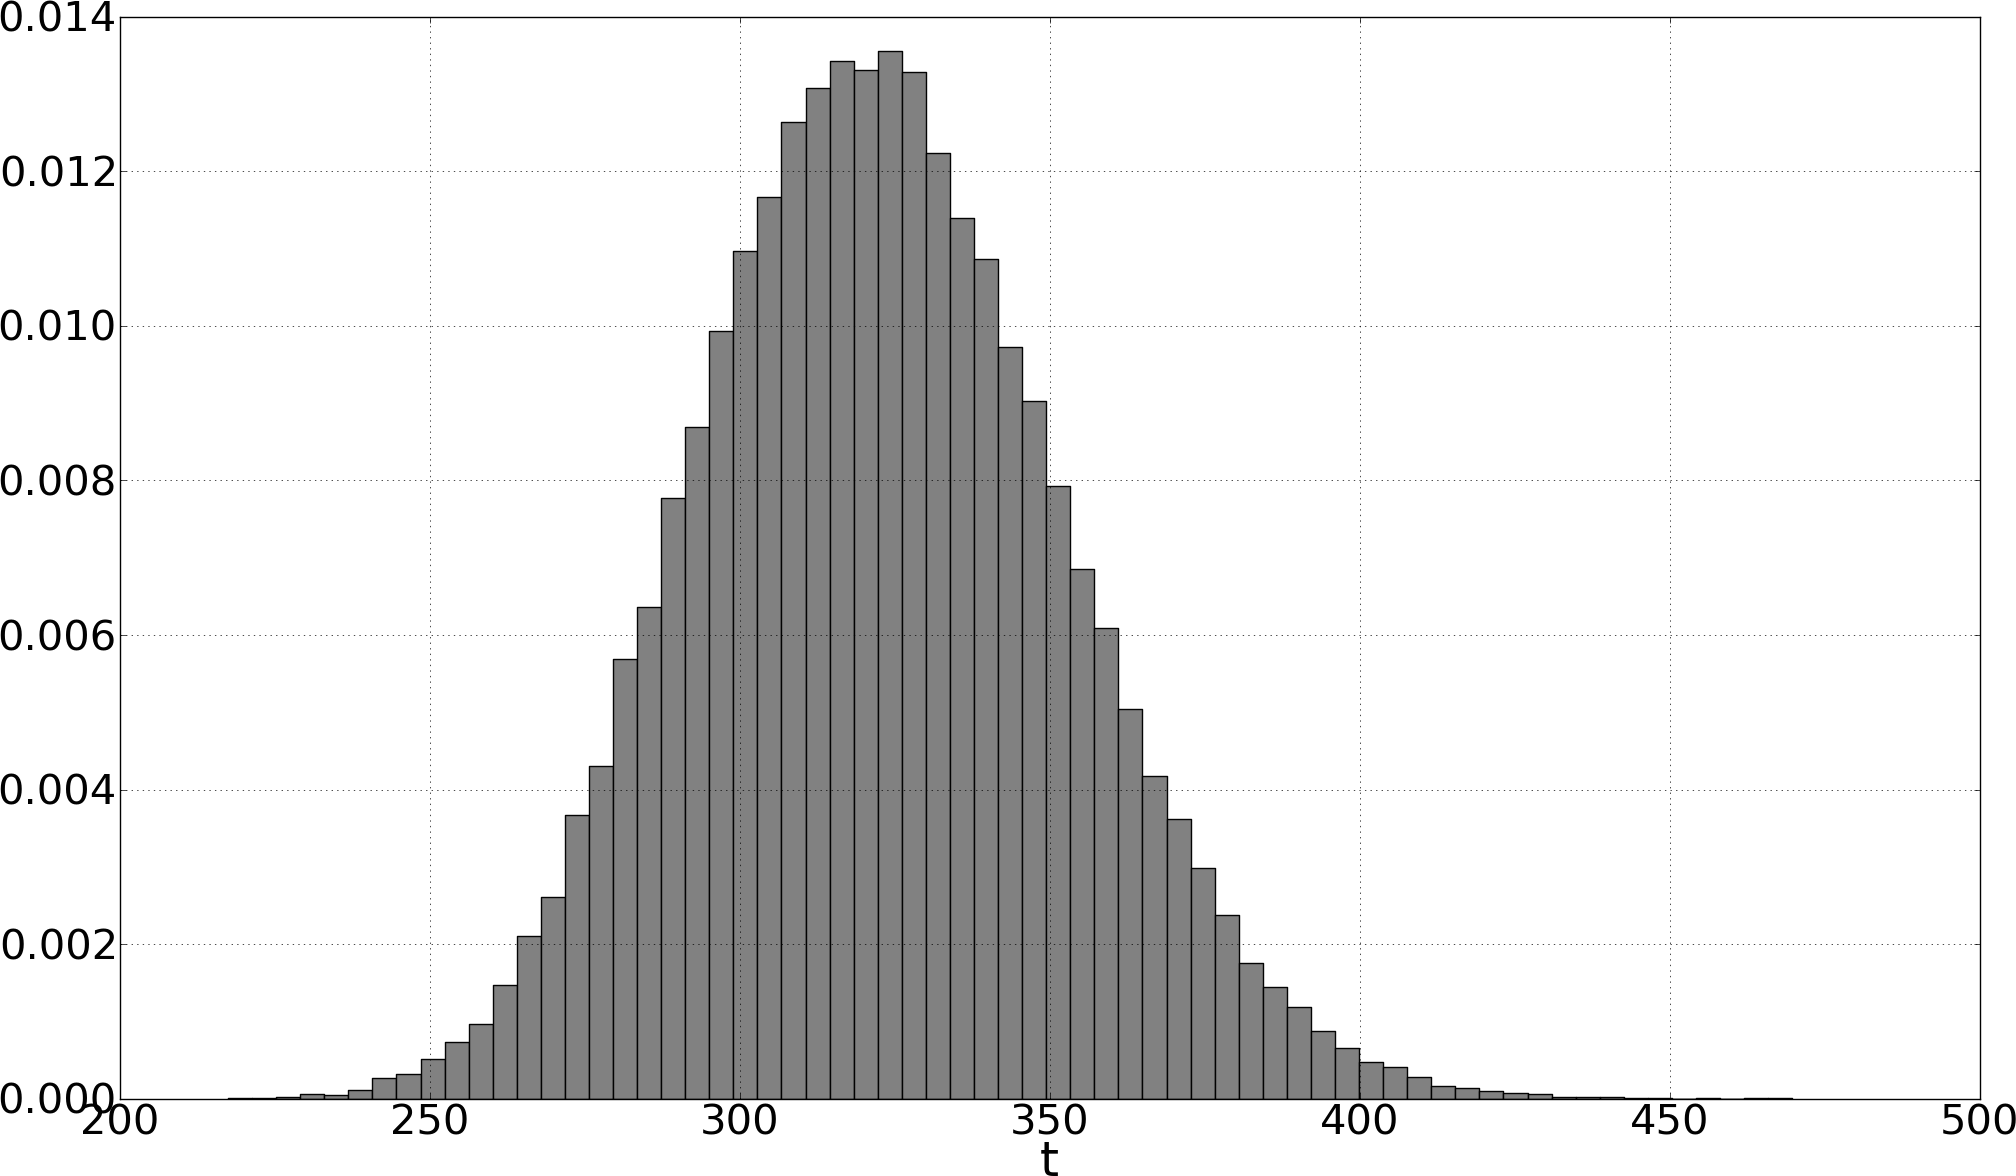
\includegraphics[width=.98\columnwidth]{58.png}
\caption{A plot of the simulated density of the test statistic for 
Problem 58. This density appears to be non-negative and slightly 
right-skew; similar to a Gamma distribution.}
\end{figurehere}
\end{homeworkProblem}

\begin{homeworkProblem}
It is given that $Z_1 , \ldots ,Z_n \sim N\left( {\mu _i ,\sigma ^2 } 
\right)$, with $\mu _{i > s}  = 0$ for some fixed known number 
$0<s<n$. It is required to find a generalized likelihood ratio test 
for:
\[
\begin{array}{*{20}c}
   {H:\mu _1  \leqslant \mu _1^0 } & {{\text{vs}}{\text{.}}} & {K:\mu 
_1  > \mu _1^0 }  \\

 \end{array} 
\]
The likelihood function is computed as:
\[
L = \left[ {\prod\limits_{i = 1}^s {\frac{1}
{{\sqrt {2\pi \sigma ^2 } }}\exp \left\{ { - \frac{1}
{{2\sigma ^2 }}\left( {z_i  - \mu _i } \right)^2 } \right\}} } 
\right]\left[ {\prod\limits_{j = s + 1}^n {\frac{1}
{{\sqrt {2\pi \sigma ^2 } }}\exp \left\{ { - \frac{1}
{{2\sigma ^2 }}z_j^2 } \right\}} } \right]
\]
\[
 = \left( {2\pi \sigma ^2 } \right)^{ - \frac{s}
{2}} \exp \left\{ { - \frac{1}
{{2\sigma ^2 }}\sum\limits_{i = 1}^s {\left( {z_i  - \mu _i } 
\right)^2 } } \right\}\left( {2\pi \sigma ^2 } \right)^{ - \frac{{n - 
s}}
{2}} \exp \left\{ { - \frac{1}
{{2\sigma ^2 }}\sum\limits_{j = s + 1}^n {z_j^2 } } \right\}
\]
\[
 = \left( {2\pi \sigma ^2 } \right)^{ - \frac{s}
{2} - \frac{{n - s}}
{2}} \exp \left\{ { - \frac{1}
{{2\sigma ^2 }}\sum\limits_{i = 1}^s {\left( {z_i  - \mu _i } 
\right)^2  - \frac{1}
{{2\sigma ^2 }}\sum\limits_{j = s + 1}^n {z_j^2 } } } \right\}
\]
\[
 = \left( {2\pi \sigma ^2 } \right)^{ - \frac{n}
{2}} \exp \left\{ { - \frac{1}
{{2\sigma ^2 }}\left[ {\sum\limits_{i = 1}^s {\left( {z_i  - \mu _i } 
\right)^2 }  + \sum\limits_{j = s + 1}^n {z_j^2 } } \right]} \right\}
\]
The log-likelihood function is therefore:
\[
LL =  - \frac{n}
{2}\ln \left( {2\pi } \right) - \frac{n}
{2}\ln \left( {\sigma ^2 } \right) - \frac{1}
{{2\sigma ^2 }}\left[ {\sum\limits_{i = 1}^s {\left( {z_i  - \mu _i } 
\right)^2 }  + \sum\limits_{j = s + 1}^n {z_j^2 } } \right]
\]
The MLEs $\hat \mu _1 , \ldots ,\hat \mu _s ,\hat \sigma ^2$ are 
therefore determined by:
\[
\frac{{\partial LL}}
{{\partial \mu _1 }} = 0 \Rightarrow  - 2z_1  - 2\mu _1  = 0 
\Rightarrow \hat \mu _1  = z_1 
\]
\[
 \vdots 
\]
\[
\frac{{\partial LL}}
{{\partial \mu _s }} = 0 \Rightarrow  - 2z_s  - 2\mu _s  = 0 
\Rightarrow \hat \mu _s  = z_s 
\]
\[
\frac{{\partial LL}}
{{\partial \sigma ^2 }} = 0 \Rightarrow \hat \sigma ^2  = 
\frac{{\sum\limits_{i = 1}^s {\left( {z_i  - \hat \mu _i } \right)^2 }  
+ \sum\limits_{j = s + 1}^n {z_j^2 } }}
{n} = \frac{1}
{n}\sum\limits_{j = s + 1}^n {z_j^2 } 
\]
The MLEs $\tilde \mu _1 , \ldots ,\tilde \mu _s ,\tilde \sigma ^2$ 
subject to the constraint ${\mu _1  \leqslant \mu _1^0 }$ are 
determined by:
\[
\frac{{\partial LL}}
{{\partial \mu _1 }} = 0 \Rightarrow  - 2z_1  - 2\mu _1  = 0,\mu _1  
\leqslant \mu _1^0  \Rightarrow \tilde \mu _1  = \mu _1^0 
\]
\[
\frac{{\partial LL}}
{{\partial \mu _2 }} = 0 \Rightarrow  - 2z_2  - 2\mu _2  = 0 
\Rightarrow \tilde \mu _2  = z_2 
\]
\[
 \vdots 
\]
\[
\frac{{\partial LL}}
{{\partial \mu _s }} = 0 \Rightarrow  - 2z_s  - 2\mu _s  = 0 
\Rightarrow \tilde \mu _s  = z_s 
\]
\[
\frac{{\partial LL}}
{{\partial \sigma ^2 }} = 0 \Rightarrow \tilde \sigma ^2  = 
\frac{{\sum\limits_{i = 1}^s {\left( {z_i  - \hat \mu _i } \right)^2 }  
+ \sum\limits_{j = s + 1}^n {z_j^2 } }}
{n} = \frac{1}
{n}\left[ {\left( {z_1  - \mu _1^0 } \right)^2  + \sum\limits_{j = s + 
1}^n {z_j^2 } } \right]
\]
Since we are interested in establishing the criteria for rejection of 
$H$, we disregard the situations where $\mu _1^0  > z_1  \Rightarrow 
\tilde \mu _1  = z_1 $; since this will lead to $\Lambda=1$ and we 
would fail to reject $H$ for any such case. Forming the likelihood 
ratio gives us:
\[
\Lambda  = \frac{{L\left( {\tilde \mu _1 , \ldots ,\tilde \mu _s 
,\tilde \sigma ^2 } \right)}}
{{L\left( {\hat \mu _1 , \ldots ,\hat \mu _s ,\hat \sigma ^2 } 
\right)}} = \frac{{\left( {2\pi \frac{1}
{n}\left[ {\left( {z_1  - \mu _1^0 } \right)^2  + \sum\limits_{j = s + 
1}^n {z_j^2 } } \right]} \right)^{ - \frac{n}
{2}} \exp \left\{ { - \frac{n}
{2}} \right\}}}
{{\left( {2\pi \frac{1}
{n}\sum\limits_{j = s + 1}^n {z_j^2 } } \right)^{ - \frac{n}
{2}} \exp \left\{ { - \frac{n}
{2}} \right\}}}
\]
\[
 = \frac{{\left( {\left( {z_1  - \mu _1^0 } \right)^2  + 
\sum\limits_{j = s + 1}^n {z_j^2 } } \right)^{ - \frac{n}
{2}} }}
{{\left( {\sum\limits_{j = s + 1}^n {z_j^2 } } \right)^{ - \frac{n}
{2}} }} = \left( {\frac{{\left( {z_1  - \mu _1^0 } \right)^2 }}
{{\sum\limits_{j = s + 1}^n {z_j^2 } }} + 1} \right)^{ - \frac{n}
{2}} 
\]
The decision rule is to reject $H$ if $\Lambda  < c \le 1$, where $c$ 
is uniquely determined by $P\left( {\Lambda  < c  } \right) = \alpha$ 
for a predetermined significance level $\alpha$. Simplification by 
division and multiplication of constant factors gives the rule for 
rejection:
\[
\left( {\frac{{\left( {z_1  - \mu _1^0 } \right)^2 }}
{{\sum\limits_{j = s + 1}^n {z_j^2 } }} + 1} \right)^{ - \frac{n}
{2}}  < c \Rightarrow \frac{{\left( {z_1  - \mu _1^0 } \right)^2 }}
{{\sum\limits_{j = s + 1}^n {z_j^2 } }} + 1 < c' \Rightarrow 
\frac{{\left( {z_1  - \mu _1^0 } \right)^2 }}
{{\sum\limits_{j = s + 1}^n {z_j^2 } }} < c''
\]
Since ${z_1  - \mu _1^0 }$  and each $z_j$ is normally distributed, 
our test statistic is recognized as having a $T$ distribution (through 
proper normalization):
\[
\frac{{\left( {z_1  - \mu _1^0 } \right)^2 }}
{{\frac{1}
{{n - s}}\sum\limits_{j = s + 1}^n {z_j^2 } }} \to \frac{{z_1  - \mu 
_1^0 }}
{{\sqrt {\frac{1}
{{n - s - 1}}\sum\limits_{j = s + 1}^n {z_j^2 } } }} \to \frac{Z}
{{\sqrt {V/d} }}\sim T\left( {n - s - 1} \right)
\]

Therefore, our test is to reject $H$ in favor of $K$ if $\phi \left( 
{Z_1 , \ldots ,Z_n } \right) = 1$, for $\phi$ defined as: 
\[
\phi \left( {Z_1 , \ldots ,Z_n } \right) = \left\{ 
{\begin{array}{*{20}c}
   1 & {\frac{{z_1  - \mu _1^0 }}
{{\sqrt {\frac{1}
{{n - s - 1}}\sum\limits_{j = s + 1}^n {z_j^2 } } }} < c,{\text{ for 
}}c{\text{ such that }}1 - \int_\infty ^c {f_T } dt = \alpha }  \\
   0 & {o.w.}  \\

 \end{array} } \right.
\]

where $f_T$ is the density of the Student's $T$ distribution with $n-
s-1$ degrees of freedom, and $\alpha$ is the chosen level of 
significance for the test.
The density of the test statistic is estimated in Fig. 4.
\begin{figurehere}
\centering
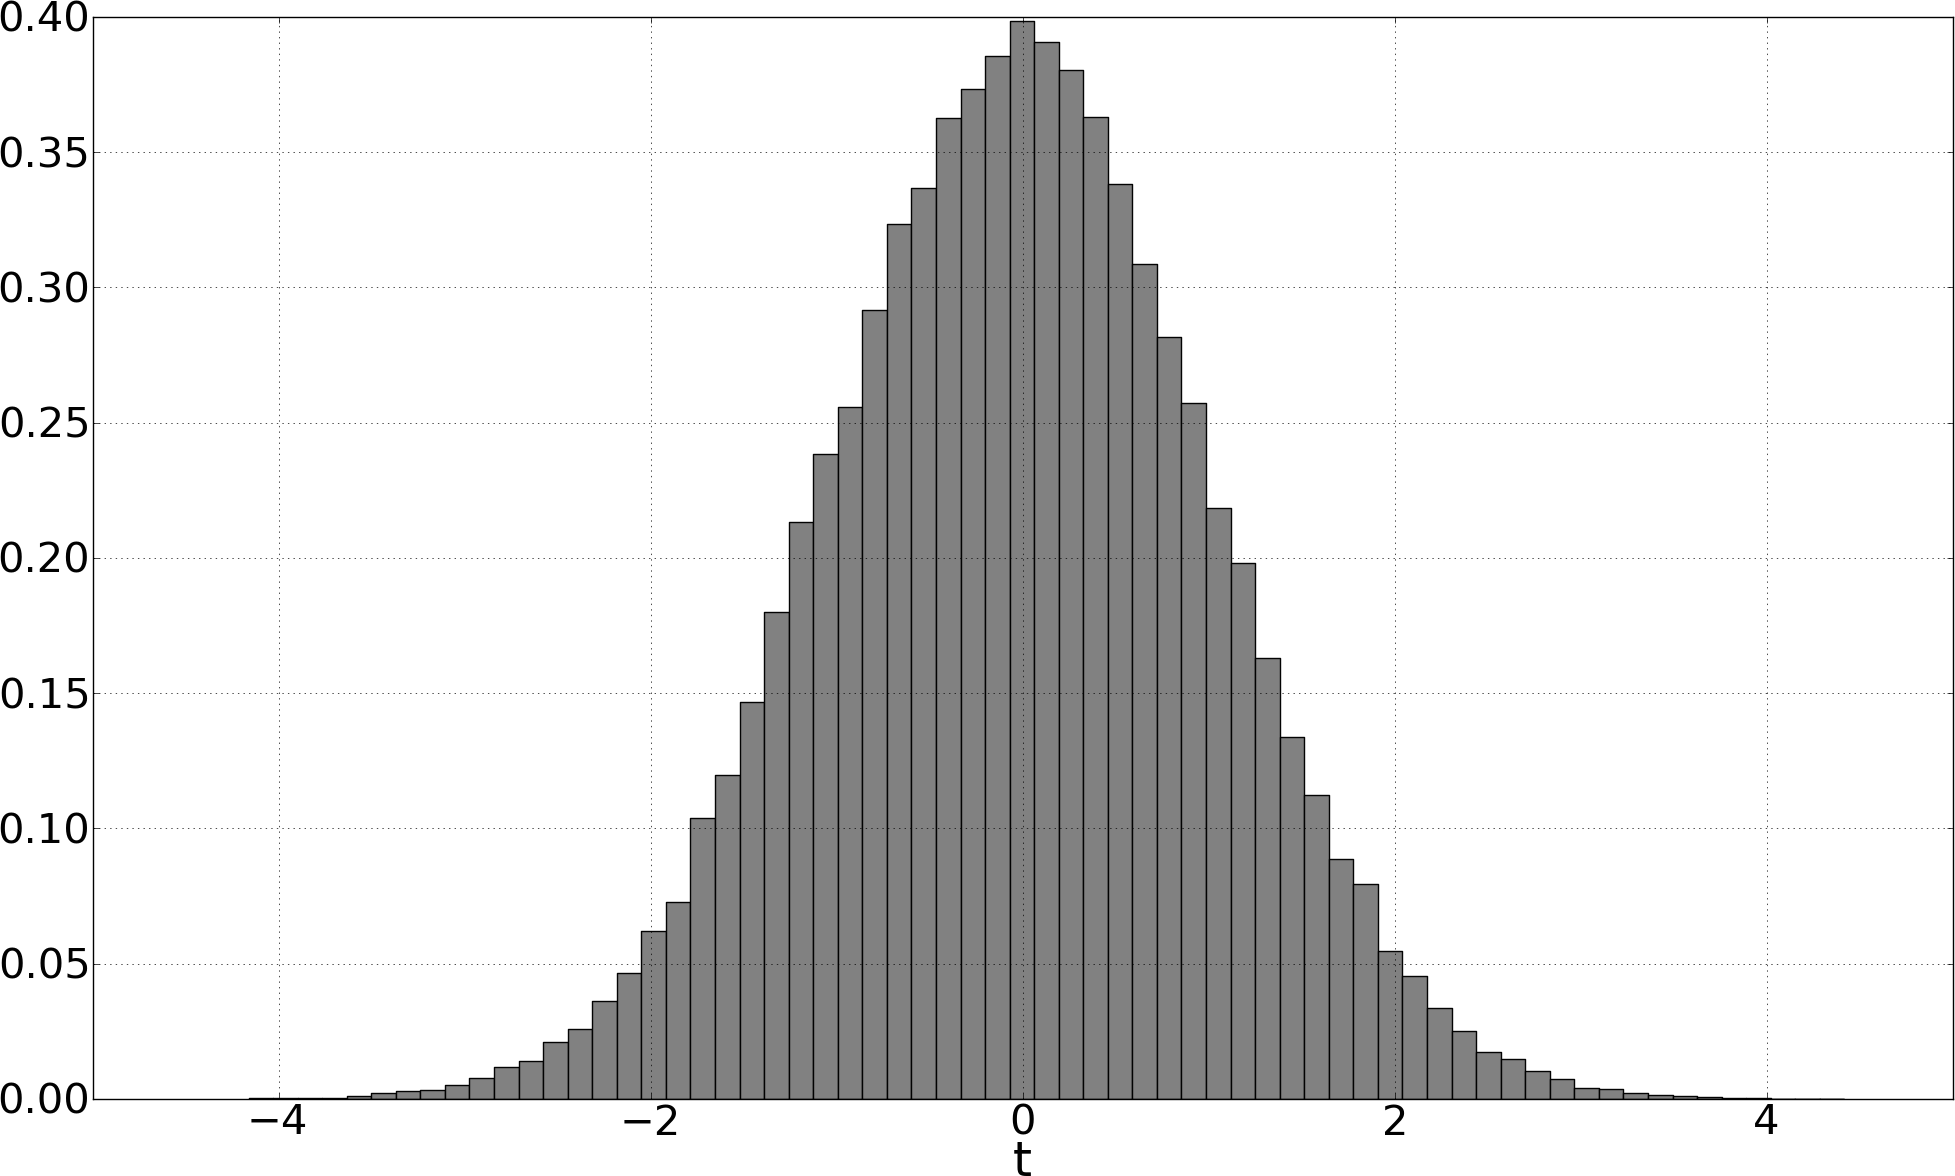
\includegraphics[width=.9\columnwidth]{59.png}
\caption{A plot of the simulated density of the test statistic for 
Problem 59. As expected, this appears to have the shape of a $T-
$distribution.}
\end{figurehere}
\end{homeworkProblem}

\begin{homeworkProblem}
Let $X_1 , \ldots ,X_n \mathop \sim \limits^{i.i.d.} Exp\left( \lambda  
\right)$. It is required to find a UMP test for: 
\[
\begin{array}{*{20}c}
   {H:\lambda  \leqslant 1} & {{\text{vs}}{\text{.}}} & {K:\lambda  > 
1}  \\

 \end{array} 
\]
First, consider the formulation of a generalized likelihood ratio test 
for the hypotheses:
\[
\begin{array}{*{20}c}
   {H':\lambda  = \lambda _0 } & {{\text{vs}}{\text{.}}} & {K':\lambda  
= \lambda _1 }  \\

 \end{array} 
\]
$\Lambda$ is computed to be:
\[
\Lambda  = \frac{{L\left( {\lambda _0 } \right)}}
{{L\left( {\lambda _1 } \right)}} = \frac{{\prod\limits_{i = 1}^n 
{\lambda _0 \exp \left\{ { - \lambda _0 x_i } \right\}} }}
{{\prod\limits_{i = 1}^n {\lambda _1 \exp \left\{ { - \lambda _1 x_i } 
\right\}} }} = \frac{{\left( {\lambda _0 } \right)^n \exp \left\{ { - 
\lambda _0 \sum\limits_{i = 1}^n {x_i } } \right\}}}
{{\left( {\lambda _1 } \right)^n \exp \left\{ { - \lambda _1 
\sum\limits_{i = 1}^n {x_i } } \right\}}}
\]
\[
 = \left( {\lambda _0 \lambda _1 } \right)^n \exp \left\{ { - \lambda 
_0 \sum\limits_{i = 1}^n {x_i }  + \lambda _1 \sum\limits_{i = 1}^n 
{x_i } } \right\} = \left( {\lambda _0 \lambda _1 } \right)^n \exp 
\left\{ {\left( {\lambda _1  - \lambda _0 } \right)\sum\limits_{i = 
1}^n {x_i } } \right\}
\]

The decision rule is to reject $H$ if $\Lambda  < c \le 1$, where $c$ 
is uniquely determined by $P\left( {\Lambda  < c  } \right) = 
\alpha=0.05$. Simplification by division and multiplication of 
constant factors gives the rule for rejection:
\[
\left( {\lambda _0 \lambda _1 } \right)^n \exp \left\{ {\left( 
{\lambda _1  - \lambda _0 } \right)\sum\limits_{i = 1}^n {x_i } } 
\right\} < c \Rightarrow \exp \left\{ {\left( {\lambda _1  - \lambda 
_0 } \right)\sum\limits_{i = 1}^n {x_i } } \right\} < c'
\]
If we assume that $\lambda_1>\lambda_0$:
\[
 \Rightarrow \left( {\lambda _1  - \lambda _0 } \right)\sum\limits_{i 
= 1}^n {x_i }  < c'' \Rightarrow \sum\limits_{i = 1}^n {x_i }  < c'''
\]
The test statistic $\sum\limits_{i = 1}^n {x_i }$ is recognized as 
having a Gamma$(n,\lambda_0)$ distribution. Therefore, our test 
function will have the form:
\[
\phi \left( {Z_1 , \ldots ,Z_n } \right) = \left\{ 
{\begin{array}{*{20}c}
   1 & {\sum\limits_{i = 1}^n {x_i }  < c,{\text{ for }}c{\text{ such 
that }}\int_{ - \infty }^c {f_{\Gamma \left( {n,\lambda _0 } \right)} 
} dt = 0.05}  \\
   0 & {o.w.}  \\

 \end{array} } \right.
\]
where ${f_{\Gamma \left( {n,\lambda _0 } \right)} }$ is the density 
function of the Gamma distribution with parameters $n$ and 
$\lambda_0$.
The inequality will change direction if $\lambda_1<\lambda_0$. Other 
than this, it is noted that the test functions do not depend on the 
exact value of $\lambda_1$. Therefore, this test is most powerful by 
the Neyman-Pearson Lemma for tests involving alternative hypothesis of 
the form:
\[
\begin{array}{*{20}c}
   {H^* :\lambda  = 1} & {{\text{vs}}{\text{.}}} & {K^* :\lambda  > 1}  
\\

 \end{array} 
\]
Now we want to show that the power function $\pi \left( {\phi ,\lambda 
} \right) = P\left( {\sum\limits_{i = 1}^n {x_i }  < c} \right)$ is 
monotonic in $\lambda$. Since:
\[
z\sim \exp \left( \lambda  \right) \Rightarrow \lambda u\sim \exp 
\left( \lambda  \right) \Rightarrow u\sim \frac{1}
{\lambda }\exp \left( 1 \right)
\]
and a sum of exponential distributions has a Gamma distribution, we 
have:
\[
\mathop {\max }\limits_{x \leqslant 1} P\left( {\sum\limits_{i = 1}^n 
{\frac{1}
{\lambda }x_i }  < c} \right) \Rightarrow \mathop {\max }\limits_{x 
\leqslant 1} P\underbrace {\left( {\sum\limits_{i = 1}^n {x_i }  < 
\lambda c} \right)}_{P \nearrow {\text{ as }}\lambda  \nearrow 
{\text{; so monotonic}}}
\]
Due to monotonicity, we may conclude that the UMP test for:
\[
\begin{array}{*{20}c}
   {H:\lambda  \leqslant 1} & {{\text{vs}}{\text{.}}} & {K:\lambda  > 
1}  \\

 \end{array} 
\] 
is specified by the test function (decision rule):
\[
\phi \left( {Z_1 , \ldots ,Z_n } \right) = \left\{ 
{\begin{array}{*{20}c}
   1 & {\sum\limits_{i = 1}^n {x_i }  < c,{\text{ for }}c{\text{ such 
that }}\int_{ - \infty }^c {f_{\Gamma \left( {1,n} \right)} } dt = 
0.05}  \\
   0 & {o.w.}  \\

 \end{array} } \right.
\]
A plot of the estimated distribution of the test statistic is given in 
Fig. 5. The estimated value of $c$ is computed from the exact PDF of a 
Gamma$(1,n)$ distribution; shown in Fig.6.\\
\begin{figurehere}
\centering
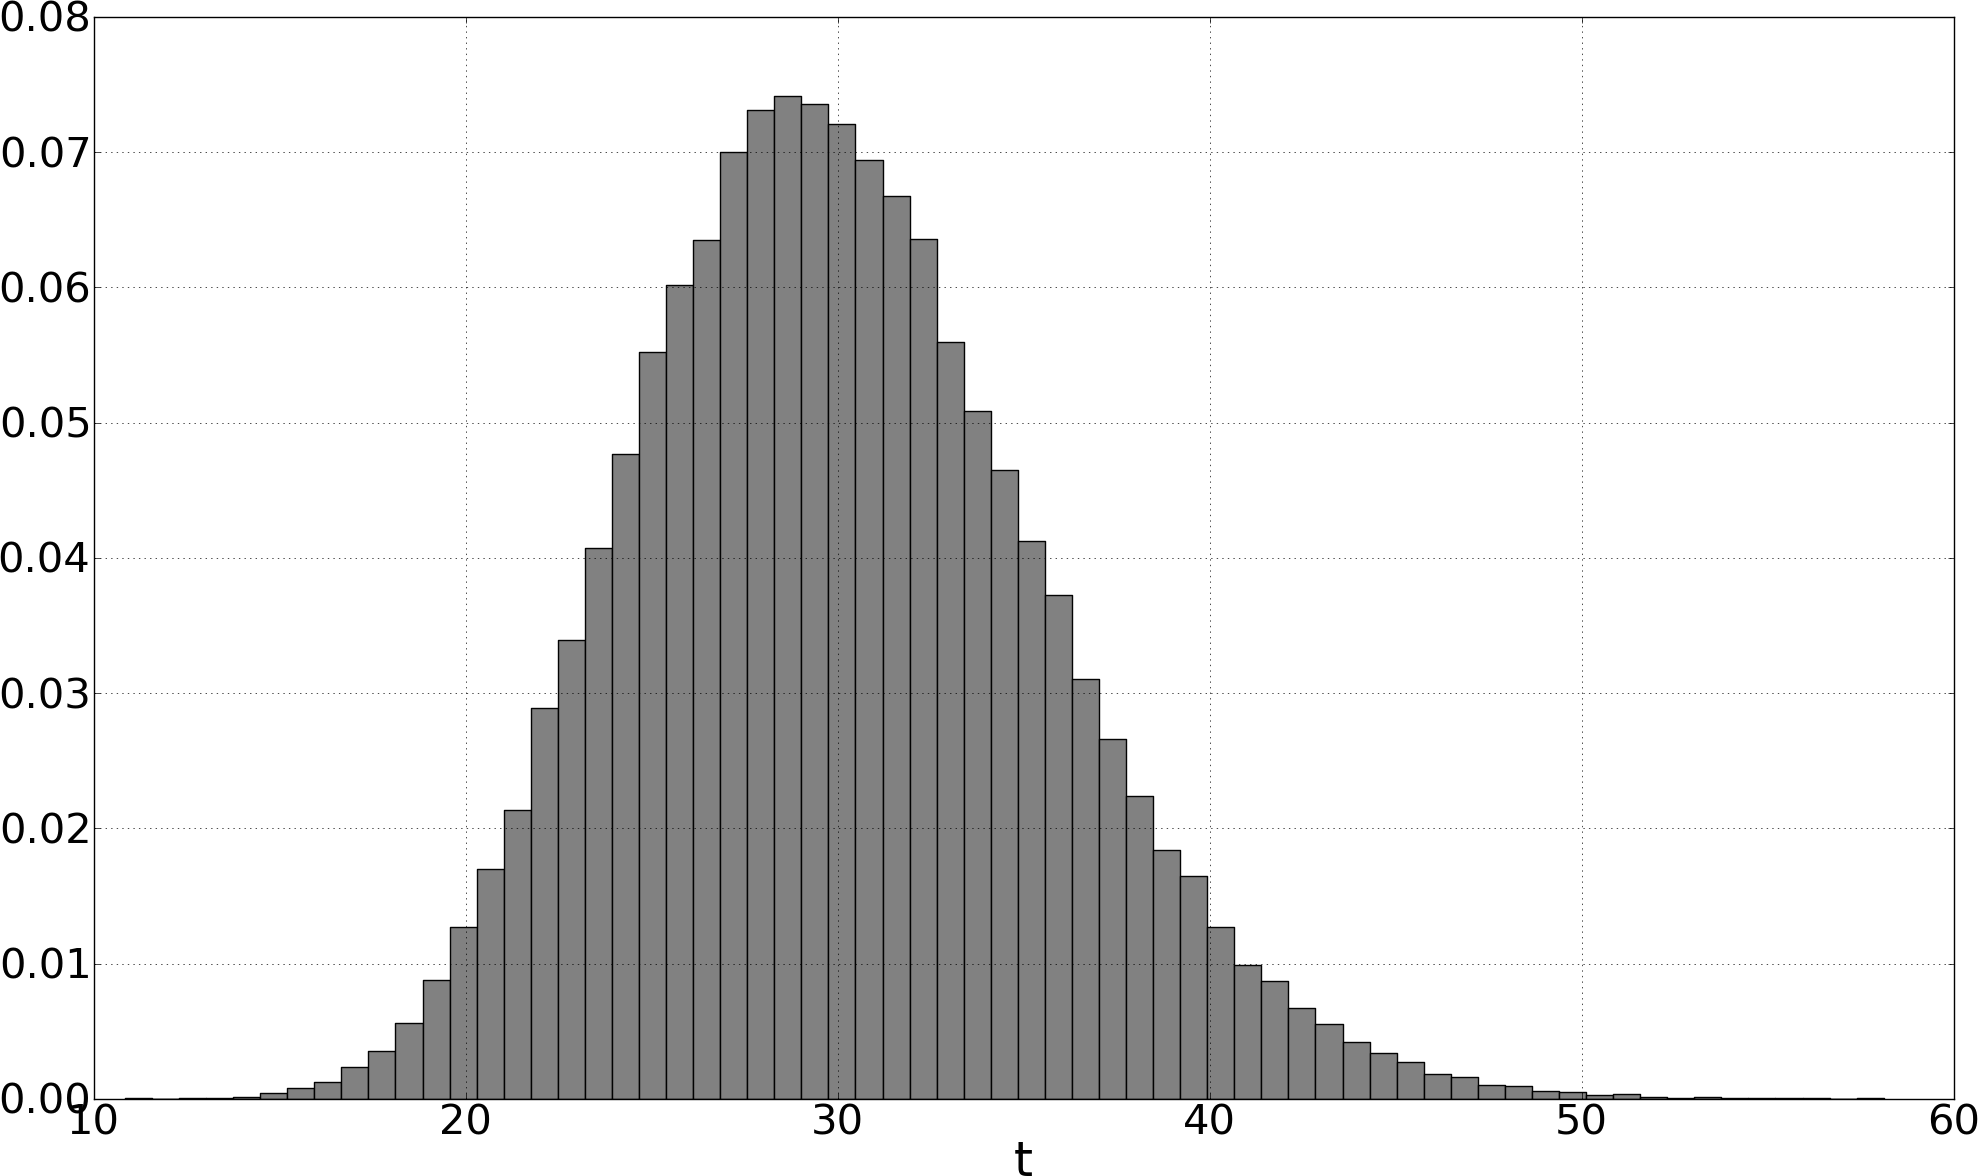
\includegraphics[width=.7\columnwidth]{60a.png}
\caption{A plot of the estimated density of the test statistic for 
Problem 60; assuming $n=30$. This appears similar to the Gamma 
distribution with parameters 1 and $n=30$, as expected.}
\end{figurehere}
\begin{figurehere}
\centering
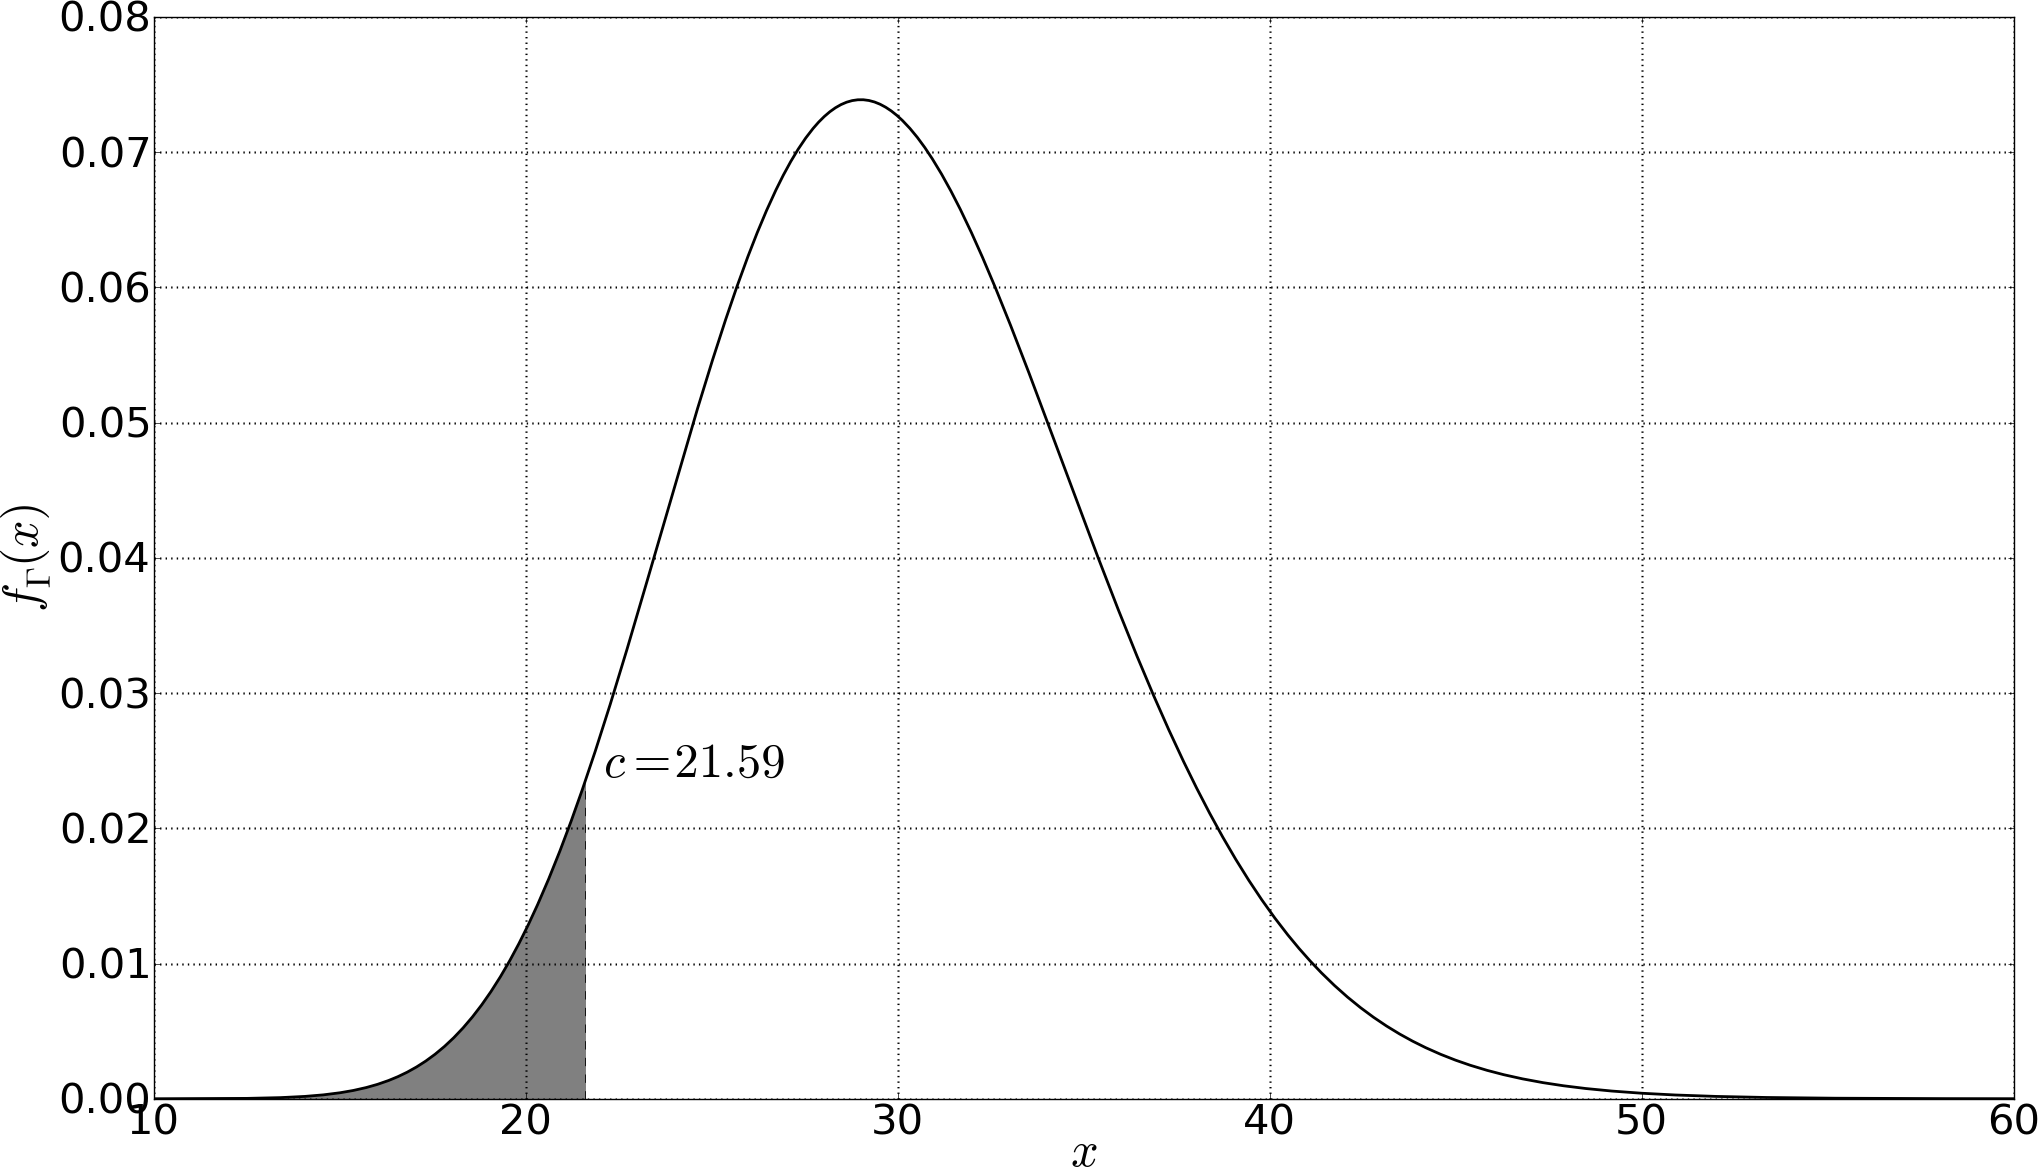
\includegraphics[width=.7\columnwidth]{60.png}
\caption{A plot of the exact density of the test statistic for Problem 
60; assuming $n=30$. This is given by the PDF of $\Gamma (1,n)$. The 
corresponding value of $c  \approx 21.59$ for $\alpha=0.05$ is also 
shown.}
\end{figurehere}
\end{homeworkProblem}
